
\documentclass[conference]{IEEEtran}

\ifCLASSINFOpdf
  \usepackage[pdftex]{graphicx}
  \graphicspath{{../pdf/}{../jpeg/}}
  \DeclareGraphicsExtensions{.pdf,.jpeg,.png}
\else
\fi

\usepackage{array}
\usepackage{pgfplots}
\pgfplotsset{compat=1.7}
\usepackage{array}
\usepackage{url}
\usepackage[T1]{fontenc}
\usepackage[utf8]{inputenc}
\usepackage{colortbl}


\hyphenation{op-tical net-works semi-conduc-tor}

\begin{document}

\title{A Survey on the Mathematical Emphasis in Brazilian Computer Science Curricula}

\author{\IEEEauthorblockN{Pedro Paulo Vezzá Campos }
\IEEEauthorblockA{Institute of Mathematics and Statistics\\
University of São Paulo\\
São Paulo, Brazil\\
Email: pedrovc@ime.usp.br}
\and
\IEEEauthorblockN{Jackson José Souza}
\IEEEauthorblockA{Institute of Mathematics and Statistics\\
University of São Paulo\\
São Paulo, Brazil\\
Email: jackson@ime.usp.br}
\and
\IEEEauthorblockN{Giuliano Salcas Olguin}
\IEEEauthorblockA{Faculty of Education\\
University of Campinas\\
Campinas, Brazil\\
Email: giuliano.olguin@gmail.com}}

\maketitle


\begin{abstract}
    A recurring question raised by professors and undergraduate students involves the distribution of basic and pratical - or professional - courses. Some authors defend a curriculum with more basic courses, such as mathematics, Physics and Chemistry, in order to create a solid background. Moreover, there is a growth of academic exchange programs all around the world, which requires a common learning base.

    Since 1960, the importance of mathematics in Computer Science (CS) undergraduate curricula has been decreasing, particularly, because new fields in CS have risen and they were assimilated in the curricula. Despite of reduction, mathematics still have its role in CS's curricula.

    The goal of this paper is to analyze the amount of the courses related to mathematics in different CS undergraduate curricula. In this work are analyzed the lecture hour load dedicated to mathematics courses on eleven Brazilian CS undergraduate programs: The Federal Universities of Ceará, Minas Gerais, Campina Grande, Pernambuco, Rio de Janeiro, Rio Grande do Sul and Santa Catarina, State Universities of São Paulo (two programs) and Campinas and the Pontifical Catholic University of Rio Grande do Sul. These programs were selected among others due their 5-stars rating in the Guia do Estudante 2012 Ranking, published by Editora Abril.

    To allow this comparison, it was established a definition of what was considered a lecture hour of mathematics. For a reference point, such programs were compared with two reference curricula in the area: The Brazilian Computer Society (SBC) and the Computer Science Curriculum 2008 made by the IEEE Computer Society and Association for Computing Machinery (ACM) joint task force.

    The curricula presented in the official sites of the selected universities in 2012 were analyzed and it was possible to conclude that more than half of the programs don't achieve the minimum amount of mathematics study hours necessary during undergraduate studies according to IEEE/ACM's reference curriculum.
\end{abstract}

\IEEEpeerreviewmaketitle

\section{Introduction}
	The recent growth of different higher education courses have resulted in a worsening of the identity crisis inside the university. Since its creation in the late thirteenth century \cite{oliveira:origem_universidades}, its function varied with the political context of local society, basically presenting values related to national issues. Still, persisted the existence of two orthogonal trends, the one which states that the University mission should be to fix the current problems of society, and the one which states that its main task is to be a beacon, glimpsing the future. The present difficulty is that there are some undergraduate programs that follow the first trend and consequently aim immediate employability by focusing on technical knowledge and others that follow the second trend, valuing the academic knowledge and being more interested in graduating professionals able to deal with problems that still doesn't exist. Merging these two powers seems to be an impossible task.
	
	According to Renato Janine, Brazilian philosopher, there are certain knowledges which are volatile, usually the technical ones, which should be taught by companies. Furthermore, it's better that in their formation years, the young deal with what's perennial, by giving him a solid foundation, than with details in constant change \cite{ribeiro:universidade_vida_atual}.

	The university should give the necessary foundations so that after graduated the person may be able to adapt to different standards used by companies in the practice of the profession whose qualification was obtained at the university. Therefore, the university should not bother to teach different types of procedures established in the labor market or teach techniques to deal only with some particular problems of the profession. In face of a rapidly changing world, where new challenges appear in an ever increasing rate, it should rather prepare students to deal with any problem or types of procedures at any time, whether present or future.

	After all, the procedures may vary not only across companies but also change over time. Thus, the trained professional would not be prepared for the future and could only adapt to companies who could handle some certain problems and only dominate some specific techniques. One can easily notice this fact through the rapid evolution of software, which require a constant learning of their manipulation, generating in some cases a disposal of knowledge previously seen.

	Therefore, it is evident that the theory and fundamentals are essential for this type of formation and can not be \emph{replaced} by just technical or practical knowledge. After all, foundations give the ability to take a given problem and use one approach or reasoning to solve it. This issue has greater impact on technology-intensive programs, such as engineering, these still being governed by entities that control the exercise of the profession.

	On the other side, practice has also an important role in the learning process. It allows students apply concepts in real problems and by this deduce conclusions which strengthen and sediments their knowledge of the area. This is particularly true for areas like Computer Science, which need to balance theory derived from algorithms concepts with programming, for example. As \cite{cs2008} states, one desirable characteristic of graduates is the appreciation of the interplay between theory and practice. ``A fundamental aspect of computer science is the balance between theory and practice and the essential link between them. Graduates of a computer science program must understand not only the theoretical underpinnings of the discipline but also how that theory
influences practice.''

	One of the common points, located in virtually every course curriculum that deal with technology are the contents of mathematics. Those, which in most cases have only a basic level of depth, precisely fit the definition that Renato Janine presented for tasks to be developed within the University. According to Anthony Ralston, mathematics develops the mind and ``improves students' learning skills.'' \cite{ralston:do_need_mathematics}

	Moreover, both Ralston and Kelemen et al \cite{kelemen:has_become_math_phobic}, are emphatic in noting that the way mathematics is offered in undergraduate programs in American universities, more specifically the Bachelor in Computer Science (BSc CS), influences on student learning.

	An important fact detected by several of the studies analyzed (\cite{ralston:do_need_mathematics}, \cite{tucker:our_curriculum_math_phobic}) is that an analysis of the reference curriculum provided by the IEEE and Association for Computing Machinery (ACM) joint task-force \cite{cs2001} \cite{cs2008} indicates that the role of mathematics has been decreasing gradually since at least the 1960s, although at a lower rate today.

	This scenario is considered bad, because for Computer Science / Software Engineering students, in particular, mathematics is important because the logical reasoning inherent in any mathematical thinking is very similar to logical thinking necessary in software development \cite{ralston:do_need_mathematics}. In developing and implementing software projects, the graduate needs to develop effective ways to solve computational problems and the amount of mathematics used in daily life of a programmer usually increases when the structures are built using a more formal language. \cite{ralston:do_need_mathematics}

	According to \cite{kelemen:has_become_math_phobic}, ``Computer Science students should be able to model `real world' problems precisely using mathematics and using structures like arrays, linked lists, trees, finite graphs and matrices. They should be able to design and analyze algorithms that transform such structures [\ldots], understand the nature of a mathematical model and relate mathematical models to areas of real problems [\ldots]. Strategies for solving problems such as divide-and-conquer and backtracking are also essential.''

	This paper aims to fill the need from university faculty who want, for example, reform their curriculum. By presenting an updated overview of the approach used in various well ranked national curricula for the math subject it is possible to make better decisions. The consolidated information is then compared with standards in the academia, allowing a broad and weighted view of the current math education reality in Brazilian CS undergraduate programs.
	
\section{Methodology}
	This paper makes a comparative study of different Brazilian Computer Science programs through a quantitative comparison of the number of lecture hours in the area of mathematics both in absolute and in relative values to the total hours required for graduation. The main goal is to identify whether the selected courses have more or less emphasis on mathematics compared with two reference curricula in the area, the Brazilian Computer Society (SBC) \cite{sbc} and the Computer Science Curriculum 2008 (CS2008) made by the IEEE Computer Society and the Association for Computing Machinery (ACM) joint task force \cite{cs2008}.

	It is important to point out, that a quantitative assessment of the hour load allows an objective classification of studided programs, on the other hand, may be less effective in analyzing the different facets that mathematics is presented in CS undergraduate courses, such as the emphasis of a particular program in the area of continuous (Calculus) or discrete mathematics (Algebra, logic, etc).

	The task of isolating covered topics or areas in different curricula, such as mathematics in this paper, for comparison purposes is on one hand very important as it enables objective analysis on the other hand is difficult to be done as different curricula have their own peculiarities. This is one of the challenges faced by accreditation organizations such as the European Network for Accreditation of Engineering Education (ENAEE), Accreditation Board for Engineering and Technology, Inc. (ABET) and the Asociación Iberoamericana de Instituciones de Enseñanza de la Ingeniería (ASIBEI). All of them are responsible for certifying that different Engineering curricula satisfy a common body of knowledge in order to facilitate students exchanges.
	

\begin{figure}[!t]
\centering
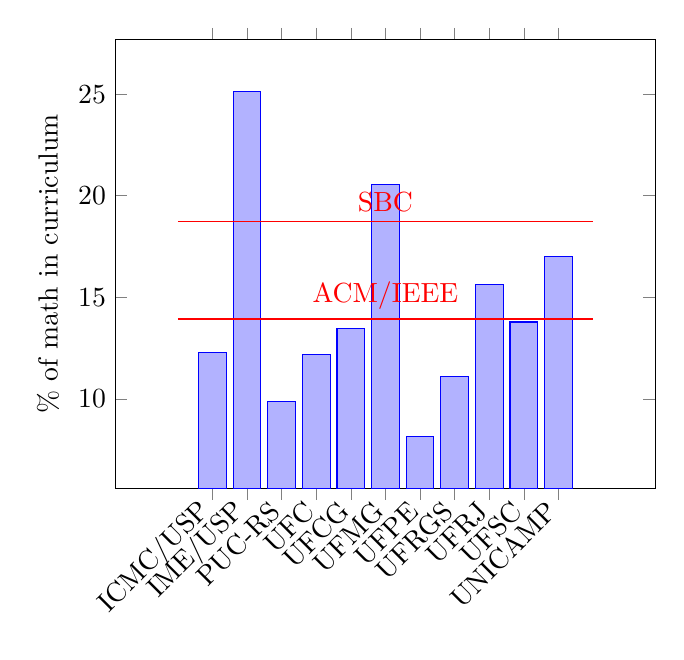
\begin{tikzpicture}
	\begin{axis}[
	ybar,
	enlargelimits=0.15,
	legend style={at={(0.5,-0.15)},
	anchor=north,legend columns=-1},
	ylabel={\% of math in curriculum},
	symbolic x coords={pre,ICMC/USP,IME/USP,PUC-RS,UFC,UFCG,UFMG,UFPE,UFRGS,UFRJ,UFSC,UNICAMP,pos},
	xtick=data,
%	nodes near coords,
%	nodes near coords align={vertical},
	x tick label style={rotate=45,anchor=east},
	]
	
	\addplot 
		coordinates {(ICMC/USP,12.29) (IME/USP,25.13) (PUC-RS,9.85) (UFC,12.20) (UFCG,13.46) (UFMG,20.57) (UFPE,8.15) (UFRGS,11.11) (UFRJ,15.61) (UFSC,13.78) (UNICAMP,17.00)};
	\addplot[red,sharp plot]
		coordinates {(pre,13.93) (pos,13.93)}
		node[above] at (axis cs:UFMG,13.93) {ACM/IEEE};
	\addplot[red,sharp plot]
		coordinates {(pre,18.75) (pos,18.75)}
		node[above] at (axis cs:UFMG,18.75) {SBC};
\end{axis}
\end{tikzpicture}
\caption{The proportion of mathematics in each curriculum compared with the reference curricula}
\end{figure}

	For this paper, are considered math disciplines those that address the areas of Calculus, Linear Algebra, Vectors, Geometry and Algebra. These subjects are usually taught by the Universities mathematics departments. A difficulty is that in some cases the names of the courses, or their syllabi, do not represent what is actually taught. All curricular material was read and classifications were created to select what in fact can be identified as mathematics.

	The ten Brazilian CS undergraduate programs studied were selected among other due to their 5-stars rating according to the Guia do Estudante 2012 Ranking, published by Editora Abril. \cite{guia_estudante} The list comprehends the Federal Universities of Ceará (UFC), Minas Gerais (UFMG), Campina Grande (UFCG), Pernambuco (UFPE), Rio de Janeiro (UFRJ), Rio Grande do Sul (UFRGS) and Santa Catarina (UFSC), State Universities of São Paulo (USP) and Campinas (UNICAMP) and the Pontifical Catholic University of Rio Grande do Sul (PUC-RS). USP is further sub-divided in two distinct CS programs, the one held at the Institute of Mathematics and Statistics (IME/USP) and the other held at the Institute of Mathematical Sciences and Computing (ICMC/USP).
	
	A side effect of this choice is that most of the programs studied are held by public universities, which must be taken into account in the data analysis since they may have different emphases in the quantity and approach in fundamentals disciplines (especially mathematics) in comparison to private universities.
	
	In 2011 the Brazilian Ministry of Education applied the latest National Test of Student Performance (ENADE) on CS programs. While some universities, like USP, chose to not participate, it presents a fairly accurate estimate on how many CS programs are in Brazil. According to it, there are at least 354 programs, 258 private and 96 public. \cite{enade} 

\section{Reference Curricula}
	As pointed out previously, Brazilian CS programs have their curricular contents mainly guided by two reference curricula. In an international level by the ACM/IEEE Computer Science Curriculum which current revision is from 2008 (CS2008) \cite{cs2008} and in a country level by the Brazilian Computer Society Curricular Reference from 2005 (CR2005) \cite{sbc}.

	CS2008 is internally subdivided in three granularities, from the bigger to the smaller: knowledge areas, knowledge units and learning objectives. The Discrete Structures (DS) knowledge area is the only one that fits (partially) in the definition of mathematics used in this paer. More specifically, DS has the following knowledge units: Functions Relations and Sets, Basic Logic, Proof Techniques, Basics of Counting, Discrete Probability, Graphs and Trees. From these, all but Graphs and Trees were accounted.

	In accordance with CS2008, 280 lecture hours are necessary to comprise the whole obligatory curriculum, with the math area representing 39 lecture hours. Note that CS2008 only addresses contents closely linked to Computer Science. There are no mentions on the requirements for Calculus, Linear Algebra or Differential Equations, necessary for advanced disciplines.

	On the other side, CR2005 has a more broad definition of mathematics than the used in this paper. It states that the following topics fall in the area: Linear Algebra, Combinatorial Analysis, Differential and Integral Calculus, Differential Equations, Analytical Geometry, Mathematical Logic, Discrete Mathematics, Probability and Statistics and Complex Variables. CR2005 doesn't detail how much time each of these topics should receive, it only affirms that it's necessary 30 ``credits'', didatic activiy units, for the whole mathematics area. The full CR2005 curriculum requires at least 160 ``credits'' for 4-year programs or 200 ``credits'' for 5-year programs.

\section{Data}
	Table I presents the general panorama of the eleven chosen CS programs indicating their size and course characteristics.

	It can be seen that most programs are diurnals (Full-time), lasting between 4 and 4.5 years. It is important to notice that the relationship between a credit and its lecture hours varies between universities. There are programs like USP and the ACM/IEEE reference curriculum that consider a credit is equal to 15 hours, on the other side, UFSC, for example, adopts the ratio 1 credit = 18 hours. The SBC curriculum does not indicate what is relation is adopted and so the authors chose to consider the value of 15 hours for comparison purposes.

\begin{table}
	\centering
	\caption{Studied CS Programs Panorama}
    \begin{tabular}{|c|c|c|>{\centering\arraybackslash}m{1cm}|}
        \hline
        University             & Period     & Graduation (years) & Students per year \\ \hline
        \rowcolor[gray]{.9}
        ACM/IEEE \cite{cs2008}      & N/A        & 4               & N/A                  \\
        \rowcolor[gray]{.9}
        SBC \cite{sbc}         & N/A        & 4               & N/A                  \\ 
        \rowcolor[gray]{.9}
        SBC \cite{sbc}         & N/A        & 5               & N/A                  \\ 
        ICMC/USP \cite{icmc}   & Diurnal    & 5               & 100                  \\ 
        IME/USP \cite{ime}     & Diurnal    & 4               & 50                   \\ 
        PUC-RS \cite{pucrs}    & Nocturnal  & 4               & 60                   \\ 
        UFC \cite{ufc}         & Diurnal    & 4               & 60                   \\ 
        UFCG \cite{ufcg}       & Diurnal    & 4               & 90                   \\ 
        UFMG \cite{ufmg}       & Diurnal    & 4               & 80                   \\ 
        UFPE \cite{ufpe}       & Diurnal    & 4.5             & 100                  \\ 
        UFRGS \cite{ufrgs}     & Diurnal    & 4.5             & 100                  \\ 
        UFRJ \cite{ufrj}       & Diurnal    & 4.5             & 50                   \\ 
        UFSC \cite{ufsc}       & Diurnal    & 4               & 100                  \\ 
        UNICAMP \cite{unicamp} & Nocturnal  & 5               & 50                   \\ 
        \hline
    \end{tabular}
\end{table}

%FIXME: Remove 1st person	
	Analyzing the amount of hours column we can see that there is a great variability in the amount required by the curricula of different universities. On average 3177h are required ($ \sigma = 554h $) for 4 years programs, 3270 hours ($ \sigma = 211h $) for 4.5 years programs and 3465 h ($ \sigma = ***h $) for 5 years programs.

\begin{table}
	\centering
	\caption{math coverage in Brazilian CS curricula}
    \begin{tabular}{|c|>{\centering\arraybackslash}m{1cm}|>{\centering\arraybackslash}m{1cm}|>{\centering\arraybackslash}m{2cm}|}
        \hline
        University               & Total math hours & Total curricular hours & Percentage of math in curriculum \\ \hline
		\rowcolor[gray]{.9}
        ACM/IEEE \cite{cs2008}        & 39               & 280                    & 13.93\%                          \\ 
		\rowcolor[gray]{.9}
        SBC (4 years) \cite{sbc} & 30               & 160                    & 18.75\%                          \\ 
        ICMC/USP \cite{icmc}     & 540              & 4395                   & 12.29\%                          \\ 
        IME/USP \cite{ime}       & 750              & 2985                   & 25.13\%                          \\ 
        PUC-RS \cite{pucrs}      & 300              & 3045                   & 9.85\%                           \\ 
        UFC \cite{ufc}           & 400              & 3280                   & 12.20\%                          \\ 
        UFCG \cite{ufcg}         & 420              & 3120                   & 13.46\%                          \\ 
        UFMG \cite{ufmg}         & 540              & 2625                   & 20.57\%                          \\ 
        UFPE \cite{ufpe}         & 285              & 3495                   & 8.15\%                           \\ 
        UFRGS \cite{ufrgs}       & 360              & 3240                   & 11.11\%                          \\ 
        UFRJ \cite{ufrj}         & 480              & 3075                   & 15.61\%                          \\ 
        UFSC \cite{ufsc}         & 486              & 3528                   & 13.78\%                          \\ 
        UNICAMP \cite{unicamp}   & 510              & 3000                   & 17.00\%                          \\
        \hline
    \end{tabular}
\end{table}

	Table 2 deals with the mathematics disciplines. Here we can see a great diversity in the workload allocation to the subject in Brazilian CS curricula. Here, universities have an average of 15.6\% ($ \sigma = 4.77\% $) of disciplines exclusively in this area.

	In Table I, the totals shown correspond to the minimum lecture hours necessary to acheive graduation, including elective disciplines or mandatory internships when they exist.

	Still, we note that when comparing each university curriculum with IEEE/ACM reference (which claims to be the minimum necessary to cover the topic) we can see that load of 5 courses have mathematics greater or equal than the recommended and 6 programs have less. This corroborates the authors' point of view cited above who claim that mathematics is a discipline in decline in CS programs.

\section{Future works}
	In Brazil there are many undergraduate rankings available. Beyond Guia do Estudante, the ENADE ranking, for example, could be used to analyze a different set of universities. Just like Guia do Estudante, ENADE analyzes the infrastructure of the university and the level of graduation of professors but also applies a test on a subset of the freshmen and senior students in order to evaluate the knowledge acquired in the graduation years. \cite{enade_info} Using the Preliminary Concept of Course (CPC) available at \cite{enade} the 10 best ranked universities are: Federal Universities of Rio Grande do Sul (UFRGS), Goiás (UFG), Campina Grande (UFCG), the city of Rio de Janeiro (Fluminense - UFF), Minas Gerais (UFMG), Pelotas (UFPel), Viçosa (UFV) and the Pampa (UNIPAMPA) and the particular Universities of the West of São Paulo (UNOESTE) and of the North (UNINORTE). 
	
	With both comparisons another possibility is to analyze if there is a positive correlation between a highly ranked program in rankings and the amount of mathematics studied during undergraduation. If so, further investigation may be necessary in order to find if there is a relation of cause and effect between the math study and the quality of a undergraduate program.
	
	Finally, different studies are possible to measure the actual utility of a more theoretical topic in the professional life of a graduate. One possibility is to apply questionnaires to former students with the goal of identifying strengths and weaknesses of a curriculum.
	
	
\section{Conclusions}
	In this paper it was possible to see how mathematics disciplines are of great importance for a future graduate in Computer Science. It was presented that such subject is a base which needs to be robust to the development of more advanced topics which are based on it. Besides, many educators in the area of Computing with articles published in international events share that view.

	Moreover, it was noted that this area is experiencing a decline in its relevance, in part by the emergence of several new trends in the market that are absorbed in undergraduate curricula.
	
	Finally, an analysis of the current emphasis on mathematics in 11 Brazilian CS curricula from 10 different universities was conducted through the study of absolute and relative workload in the area. It was found that more than 50 \% of the programs surveyed have a lower load than recommended by ACM reference curriculum.
	
% An example of a floating figure using the graphicx package.
% Note that \label must occur AFTER (or within) \caption.
% For figures, \caption should occur after the \includegraphics.
% Note that IEEEtran v1.7 and later has special internal code that
% is designed to preserve the operation of \label within \caption
% even when the captionsoff option is in effect. However, because
% of issues like this, it may be the safest practice to put all your
% \label just after \caption rather than within \caption{}.
%
% Reminder: the "draftcls" or "draftclsnofoot", not "draft", class
% option should be used if it is desired that the figures are to be
% displayed while in draft mode.
%
%\begin{figure}[!t]
%\centering
%\includegraphics[width=2.5in]{myfigure}
% where an .eps filename suffix will be assumed under latex, 
% and a .pdf suffix will be assumed for pdflatex; or what has been declared
% via \DeclareGraphicsExtensions.
%\caption{Simulation Results}
%\label{fig_sim}
%\end{figure}

% Note that IEEE typically puts floats only at the top, even when this
% results in a large percentage of a column being occupied by floats.


% An example of a double column floating figure using two subfigures.
% (The subfig.sty package must be loaded for this to work.)
% The subfigure \label commands are set within each subfloat command, the
% \label for the overall figure must come after \caption.
% \hfil must be used as a separator to get equal spacing.
% The subfigure.sty package works much the same way, except \subfigure is
% used instead of \subfloat.
%
%\begin{figure*}[!t]
%\centerline{\subfloat[Case I]\includegraphics[width=2.5in]{subfigcase1}%
%\label{fig_first_case}}
%\hfil
%\subfloat[Case II]{\includegraphics[width=2.5in]{subfigcase2}%
%\label{fig_second_case}}}
%\caption{Simulation results}
%\label{fig_sim}
%\end{figure*}
%
% Note that often IEEE papers with subfigures do not employ subfigure
% captions (using the optional argument to \subfloat), but instead will
% reference/describe all of them (a), (b), etc., within the main caption.



% An example of a floating table. Note that, for IEEE style tables, the 
% \caption command should come BEFORE the table. Table text will default to
% \footnotesize as IEEE normally uses this smaller font for tables.
% The \label must come after \caption as always.
%
%\begin{table}[!t]
%% increase table row spacing, adjust to taste
%\renewcommand{\arraystretch}{1.3}
% if using array.sty, it might be a good idea to tweak the value of
% \extrarowheight as needed to properly center the text within the cells
%\caption{An Example of a Table}
%\label{table_example}
%\centering
%% Some packages, such as MDW tools, offer better commands for making tables
%% than the plain LaTeX2e tabular which is used here.
%\begin{tabular}{|c||c|}
%\hline
%One & Two\\
%\hline
%Three & Four\\
%\hline
%\end{tabular}
%\end{table}




% trigger a \newpage just before the given reference
% number - used to balance the columns on the last page
% adjust value as needed - may need to be readjusted if
% the document is modified later
%\IEEEtriggeratref{8}
% The "triggered" command can be changed if desired:
%\IEEEtriggercmd{\enlargethispage{-5in}}

\bibliographystyle{IEEEtran}
\bibliography{bibliography}


\end{document}

